\chapter{Manipulação de Dados no Jamovi}

O foco deste capítulo é a manipulação de dados, uma habilidade essencial para qualquer pessoa que esteja interessada em análise de dados. Vamos explorar as diversas funções e recursos do Jamovi para tratar, organizar e manipular conjuntos de dados. Se você já se perguntou como criar e gerenciar categorias, transformar dados ou manipular variáveis no Jamovi, este capítulo irá te guiar através desses processos passo a passo.

No capítulo anterior você deu os primeiros passos e apresentamos a você a interface do Jamovi para manipulação de dados. Nesse capítulo discutiremos o fluxo de trabalho ideal para o tratamento de um conjunto de dados. O objetivo é garantir que você tenha uma compreensão sólida das ferramentas disponíveis e de como usá-las eficientemente.

Em seguida, abordaremos como criar novas categorias a partir de variáveis existentes. Isso pode ser útil em uma variedade de contextos, como quando você deseja agrupar respostas de pesquisas ou classificar dados em grupos específicos. Também ensinaremos a transformar variáveis, permitindo que você mude o formato dos seus dados de uma maneira que melhor atenda às suas necessidades analíticas.

Finalmente, traremos exemplos práticos para aplicar o conhecimento adquirido. O intuito é promover a familiarização com as ferramentas do software e reforçar a compreensão das funcionalidades abordadas.

Lembre-se, a manipulação eficaz dos dados é a base de qualquer análise de qualidade. Por isso, este capítulo desempenha um papel fundamental no seu aprendizado sobre o uso do Jamovi. Esperamos que ao final desta etapa, você se sinta confiante para manipular conjuntos de dados e prepará-los para a análise de uma maneira eficiente e eficaz.

\section{Introdução à Manipulação de Dados}
Nesta seção, apresentaremos o papel crucial da manipulação de dados na análise de dados. Exploraremos seu propósito, benefícios e relevância no contexto do software Jamovi.

\section{Interface do Jamovi}
Este segmento é dedicado a apresentar a interface de manipulação de dados do Jamovi. Discutiremos os componentes visuais e explicaremos como interagir com eles para realizar diversas operações.

\section{Importação de Dados}
Aqui, abordaremos o processo de importação de dados no Jamovi. Enfatizaremos a importância de compreender diferentes formatos de dados e como manuseá-los no software.

\section{Criação de Variáveis}
Nesta seção, ensinaremos como criar novas variáveis a partir de variáveis já existentes. Essa é uma habilidade fundamental ao trabalhar com grandes conjuntos de dados.

\section{Transformação de Variáveis}
A transformação de variáveis é um aspecto essencial da manipulação de dados. Aqui, exploraremos as diferentes maneiras de transformar variáveis no Jamovi.

\section{Criação de Categorias}
Neste segmento, discutiremos como criar e gerenciar categorias no Jamovi. Isso é particularmente útil ao lidar com variáveis categóricas e dados de pesquisa.

Para ilustrar como isso é feito, usaremos o \href{https://github.com/balaio-cientifico/dataset/blob/main/pop_ts.txt}{Dataset de População - IBGE} como exemplo. Este dataset contém dados sobre a população dos municípios brasileiros, com informações coletadas nos censos de 2010 e 2022, bem como projeções populacionais realizadas pelo IBGE. Os dados de população são especialmente adequados para a criação de categorias, já que podem ser agrupados de várias maneiras.

Neste tutorial, iremos focar em como usar esse dataset para criar categorias populacionais que representam cidades grandes, médias e pequenas. Este é um exemplo comum de como os dados populacionais são categorizados para análises demográficas, urbanísticas ou sociais.

Para começar, precisamos definir quais são os critérios para uma cidade ser considerada grande, média ou pequena. Essa definição pode variar dependendo do contexto, mas para os fins deste tutorial, iremos definir as categorias da seguinte forma: cidades pequenas são aquelas com população inferior a 20.000 habitantes, cidades médias possuem entre 20.000 e 100.000 habitantes, e cidades grandes são aquelas com mais de 100.000 habitantes.\footnote{Por favor, note que essa classificação é puramente ilustrativa e serve apenas para o propósito deste tutorial. Essa divisão de categorias não possui uma base científica rigorosa e pode variar consideravelmente dependendo do contexto específico. É importante ressaltar que, em sua própria análise, você está livre para definir suas próprias categorias com base nos critérios que considerar mais relevantes para o seu estudo.}

Após a importação dos dados, o primeiro passo para criar categorias no Jamovi é utilizar a opção "Transformar Variáveis". Existem duas maneiras de acessar essa funcionalidade.

A primeira maneira é através do menu de dados. Clique no menu "Dados" na parte superior da interface do Jamovi. Em seguida, selecione a opção "Transformar". Neste ponto, você pode selecionar a variável que deseja transformar em categorias.

A segunda opção, que é um pouco mais direta, envolve clicar com o botão direito do mouse no cabeçalho da variável que você deseja transformar. No menu que aparecerá, selecione a opção "Transformar".

Essas ações são ilustradas na Figura~\ref{fig:criar_categoria_jamovi}. Essa figura indica onde você precisa clicar para acessar a opção de transformação de variáveis.

Por favor, note que a escolha do método para acessar a opção de transformação de variáveis depende da sua preferência. Ambos os métodos levam ao mesmo resultado, então você pode escolher o que achar mais conveniente.

\begin{figure}[H]
    \centering
    \caption{Selecionando a Opção Transformar no Jamovi}
    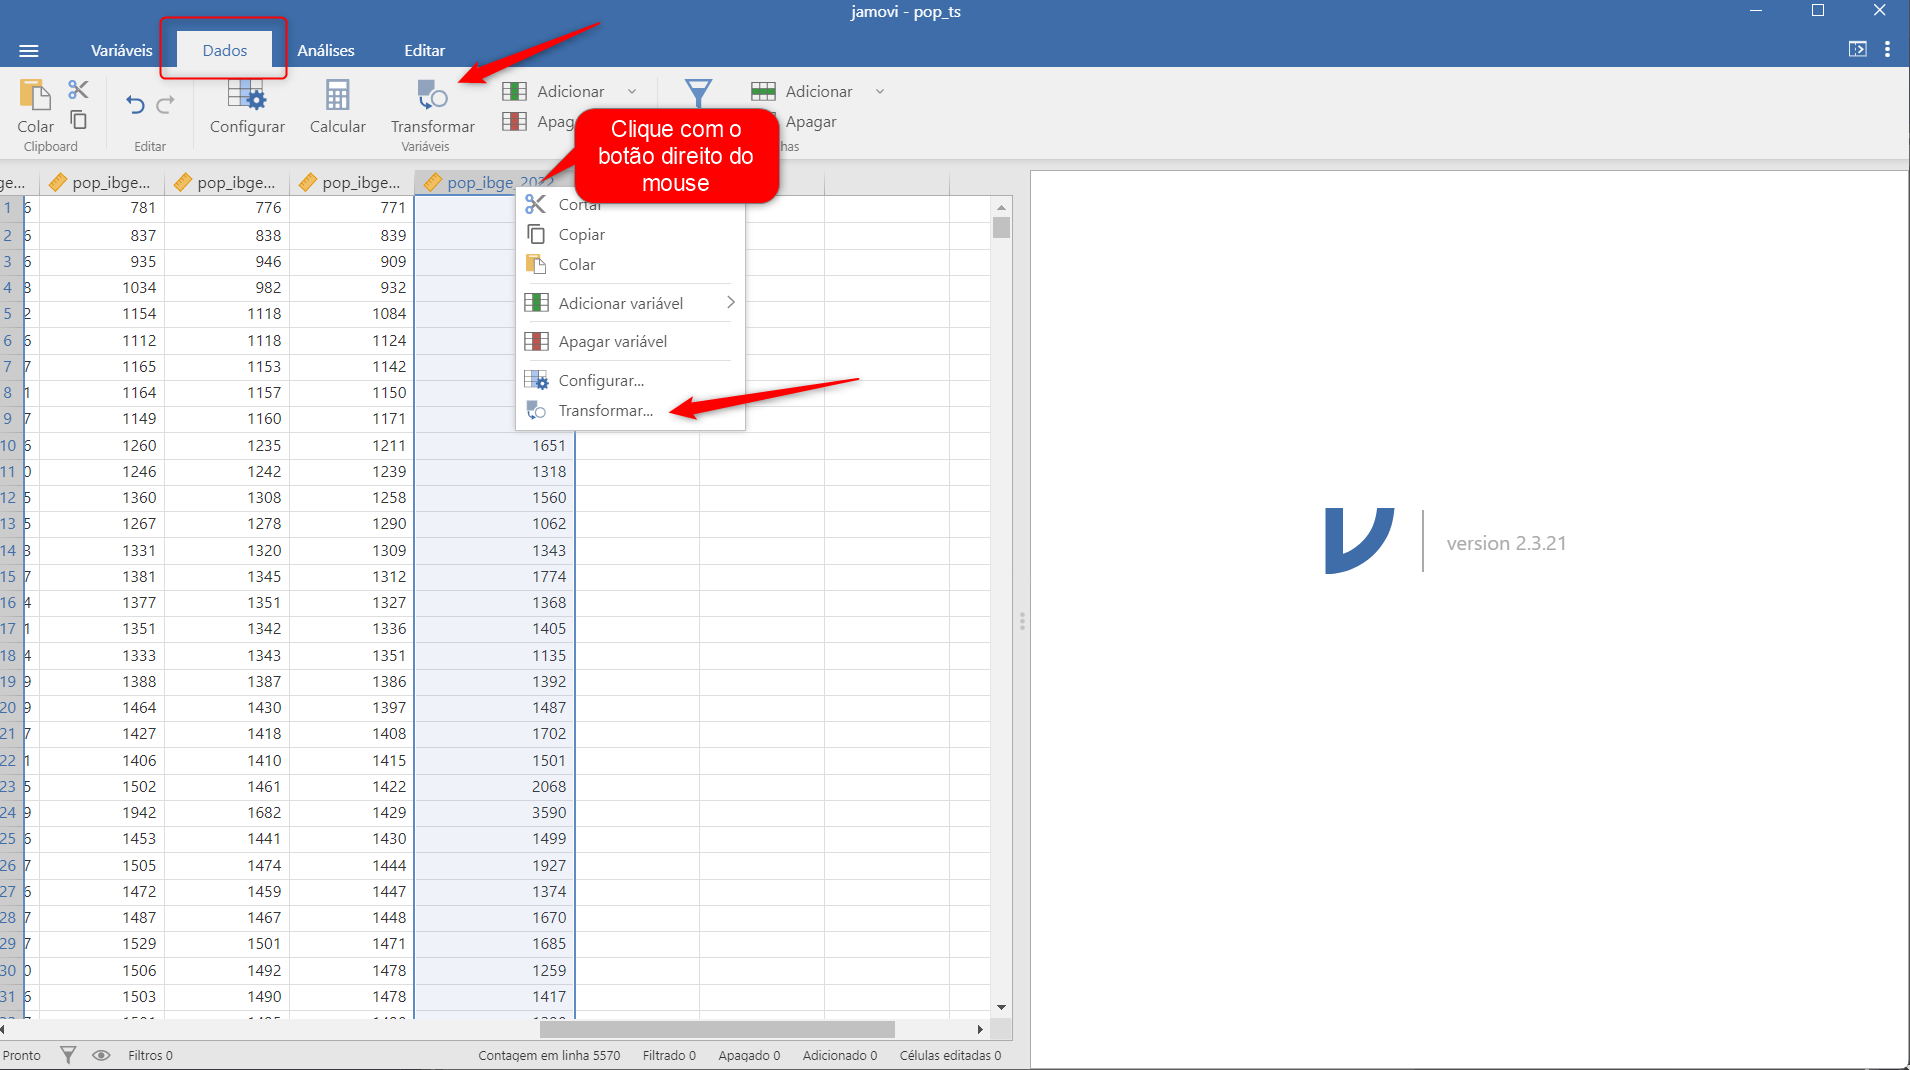
\includegraphics[width=\textwidth]{imagens/cap_2/criar_categoria_jamovi.png}
    \label{fig:criar_categoria_jamovi}
\end{figure}

No exemplo que vamos tratar neste tutorial, estaremos utilizando a variável \textit{pop\_ibge\_2022}. Esta variável refere-se à população dos municípios brasileiros conforme estimado no censo do IBGE de 2022. Esta variável contínua será transformada em uma variável categórica que representa cidades grandes, médias e pequenas, de acordo com os critérios de classificação que definimos anteriormente.

Agora, precisamos configurar a nova variável categórica que será criada. Nesta etapa, você deverá escolher um nome para a nova variável. No nosso exemplo, chamaremos essa variável de \textit{cat\_pop\_2022}, mas sinta-se livre para escolher o nome que preferir. 

Além disso, é uma boa prática incluir uma descrição para a variável, que explique brevemente o que ela representa. No nosso caso, a descrição será ``Categoria do tamanho das cidades''. Mais uma vez, sinta-se à vontade para criar uma descrição que se adeque ao seu contexto.

É importante confirmar que a variável alvo, neste caso \textit{pop\_ibge\_2022}, foi corretamente selecionada, como é mostrado na Figura~\ref{fig:criar_categoria_jamovi_2}. Essa verificação ajuda a evitar erros na transformação dos dados.

\begin{figure}[H]
    \centering
    \caption{Configurando a nova variável categoórica}
    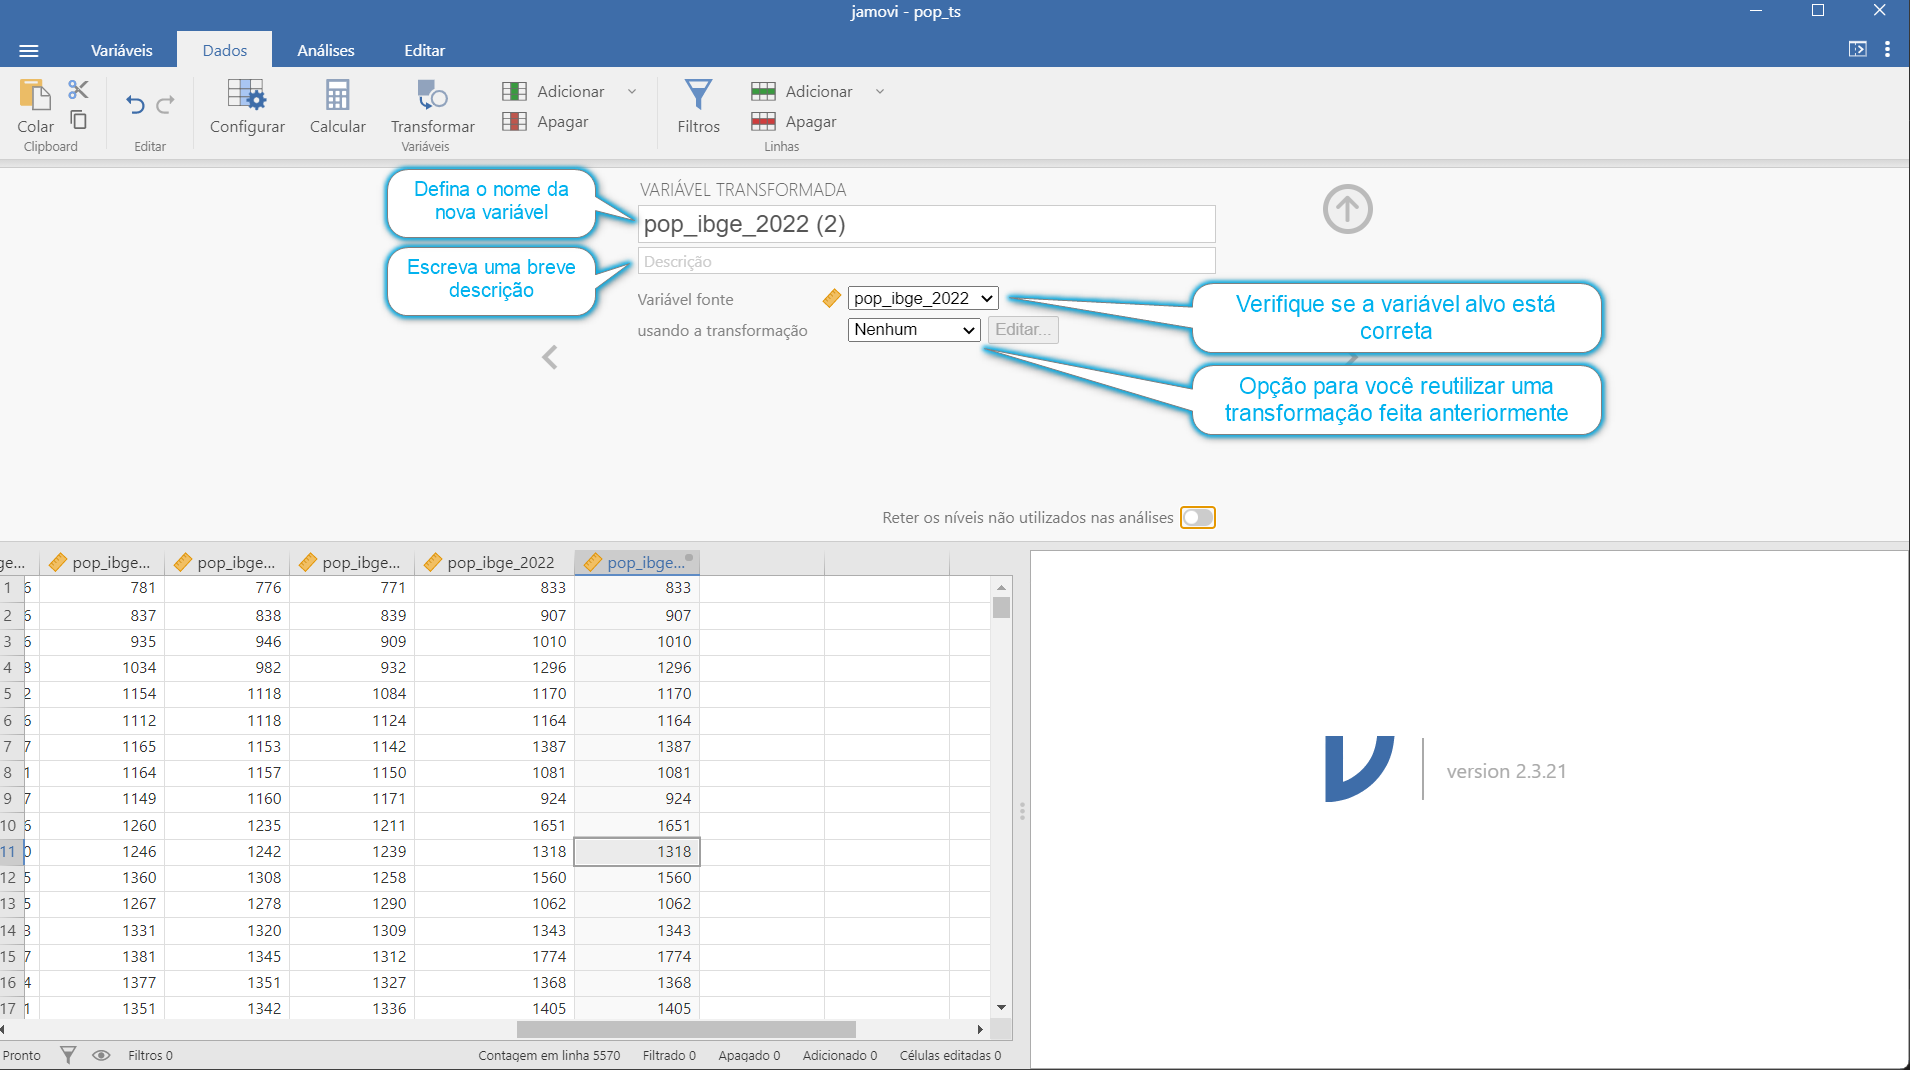
\includegraphics[width=\textwidth]{imagens/cap_2/criar_categoria_jamovi_2.png}
    \label{fig:criar_categoria_jamovi_2}
\end{figure}

Conforme pode ser observado na Figura \ref{fig:criar_categoria_jamovi_3}, a nova variável foi criada e agora precisamos configurar a transformação que será aplicada. Para isso, basta clicar no botão para adicionar uma nova transformação.

É importante salientar que estamos considerando, para fins deste tutorial, que você nunca realizou uma transformação desse tipo antes. Portanto, se este for o seu caso, não se preocupe, pois todas as etapas serão explicadas detalhadamente para auxiliá-lo(a) neste processo.

\begin{figure}[H]
    \centering
    \caption{Nova variável categórica criada}
    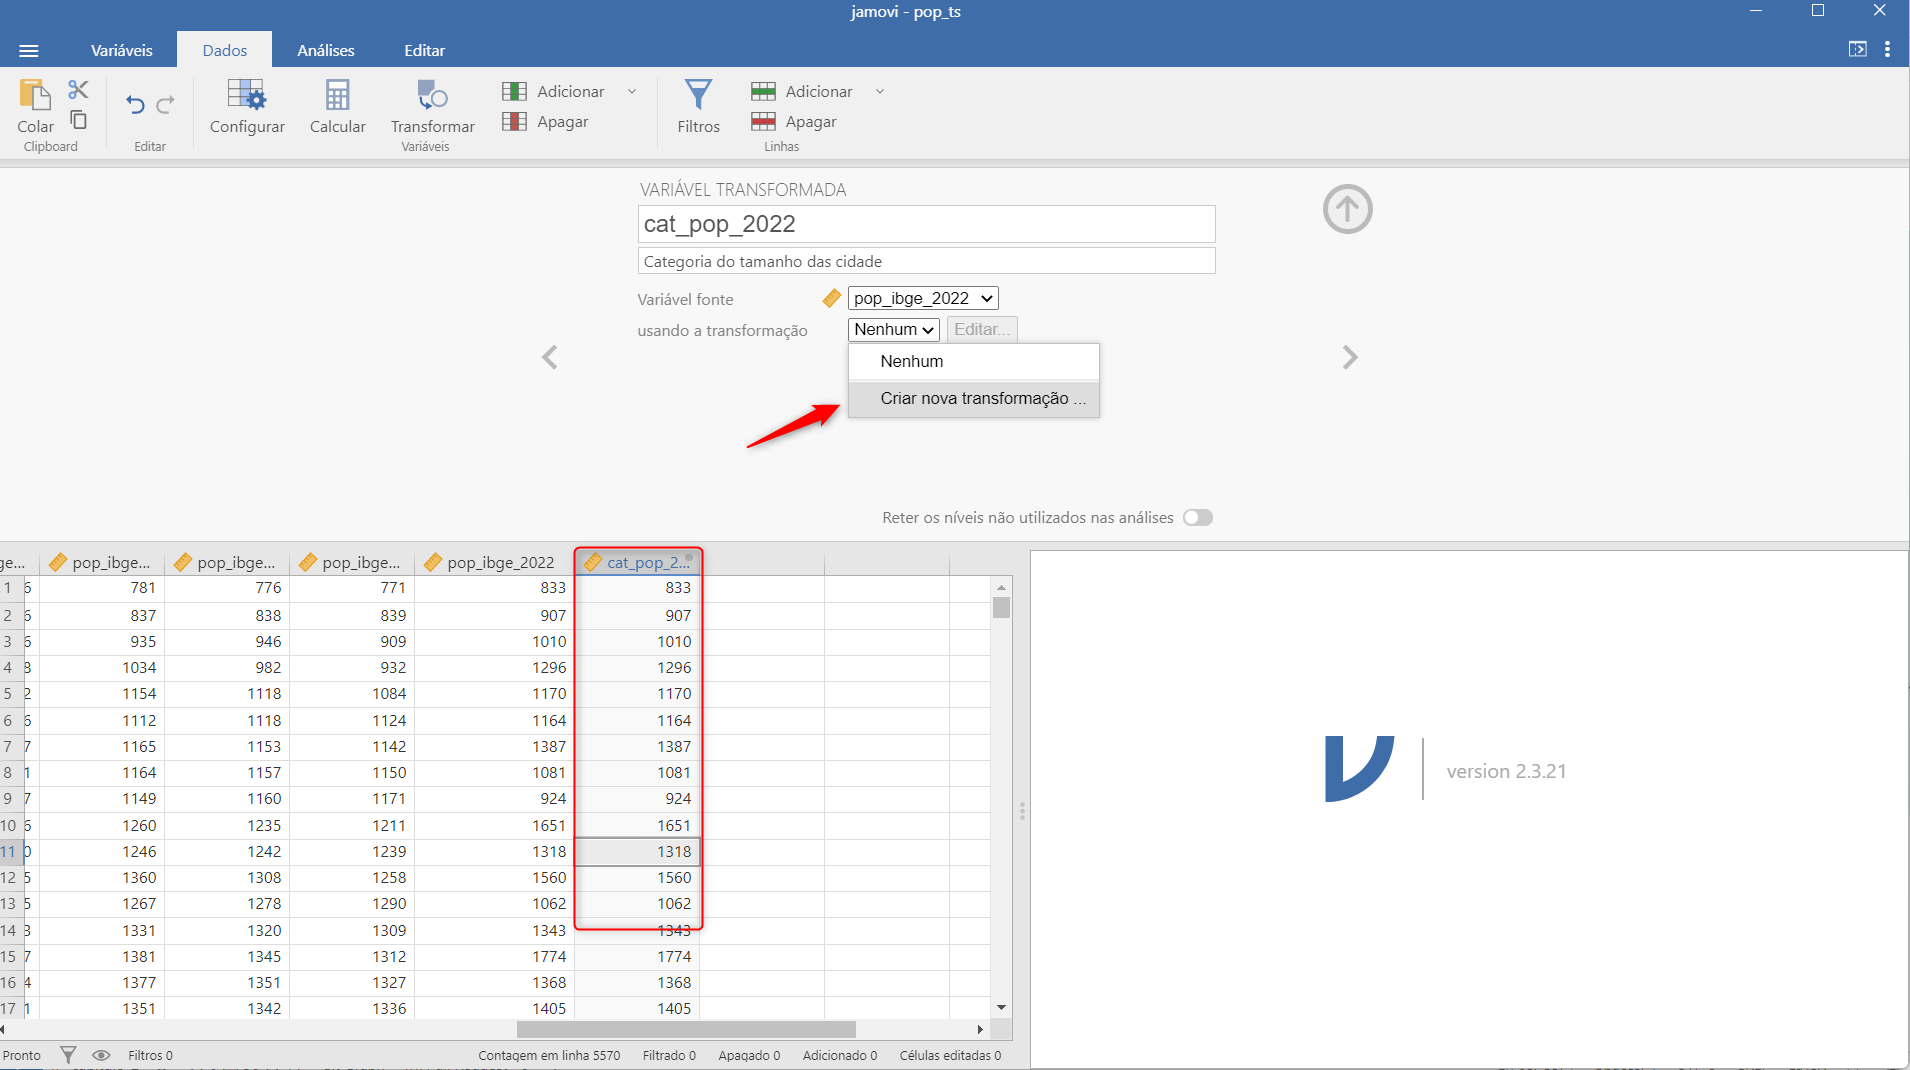
\includegraphics[width=\textwidth]{imagens/cap_2/criar_categoria_jamovi_3.png}
    \label{fig:criar_categoria_jamovi_3}
\end{figure}

Neste ponto, você deverá especificar um nome para a configuração da transformação. Esta etapa é similar à definição de uma função em programação - o Jamovi irá armazenar esta configuração que poderá ser usada posteriormente.

A Figura~\ref{fig:criar_categoria_jamovi_4} ilustra esta etapa. O primeiro campo é onde você insere o nome da transformação. Em seguida, você tem a opção de adicionar uma descrição. Embora isso seja opcional, sempre aconselho a preencher este campo para ajudar a lembrar o que a transformação faz, especialmente se você planeja compartilhar seu trabalho com outras pessoas ou se estiver trabalhando em um projeto de longo prazo.

Finalmente, o passo 3 é onde você seleciona a opção "Adicionar condição de recodificação". Esta é a etapa onde você irá definir as múltiplas condições que irão criar a sua variável categórica.

\begin{figure}[H]
    \centering
    \caption{Configura as categorias para criação das categorias}
    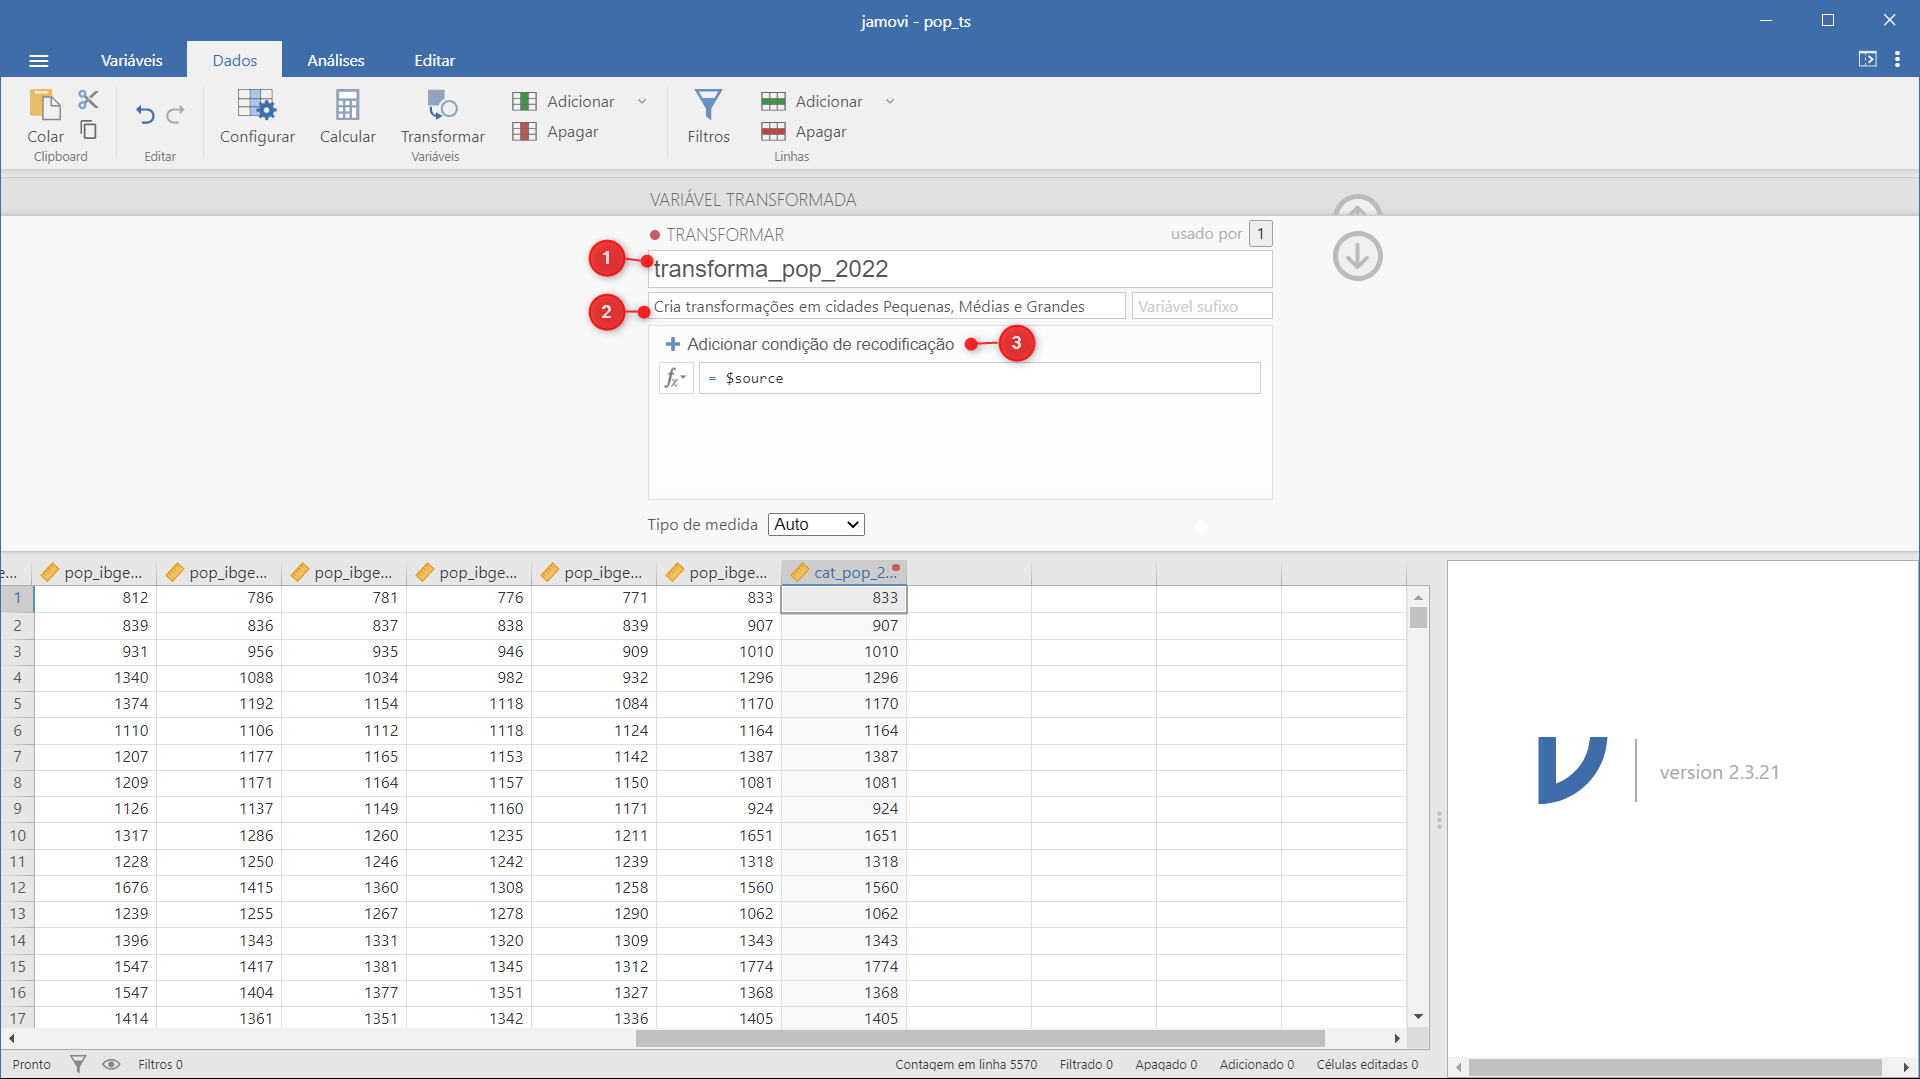
\includegraphics[width=\textwidth]{imagens/cap_2/criar_categoria_jamovi_4.png}
    \label{fig:criar_categoria_jamovi_4}
\end{figure}

Chegamos agora à fase em que iremos definir as condições para a criação da nossa variável categórica no Jamovi. Para fazer isso, precisaremos escrever expressões lógicas, um recurso muito comum em programação. 

Como dito anteriormente, o Jamovi foi construído com base na linguagem R, o que significa que muitos dos recursos de sintaxe do R são aplicáveis ao Jamovi. Portanto, uma compreensão básica da linguagem R pode ser muito útil ao usar o Jamovi.

Se você se sentir um pouco perdido(a) nesse ponto, não se preocupe! Para aqueles que desejam se aprofundar mais no uso da linguagem R e, por consequência, melhorar suas habilidades no Jamovi, recomendo o meu livro de \href{https://www.amazon.com.br/Fundamentos-Completo-Iniciantes-programa%C3%A7%C3%A3o-computa%C3%A7%C3%A3o-ebook/dp/B0B36NG18N}{Fundamentos em R: Guia Completo para Iniciantes}. Nele, eu exploro em detalhes como utilizar o R, o que pode ser de grande ajuda para aprimorar seu domínio do Jamovi.

Veja na Figura~\ref{fig:criar_categoria_jamovi_5}, o local em que você deve selecionar as condições para criarmos as categorias de cidades: pequenas, médias e grandes. Clique na seção de operadores e selecione ou escreva conforme eu escrevi na tabela \ref{fig:criar_categoria_jamovi_6}

\begin{figure}[H]
    \centering
    \caption{Seleciona a caixa para escrever as condições no Jamovi}
    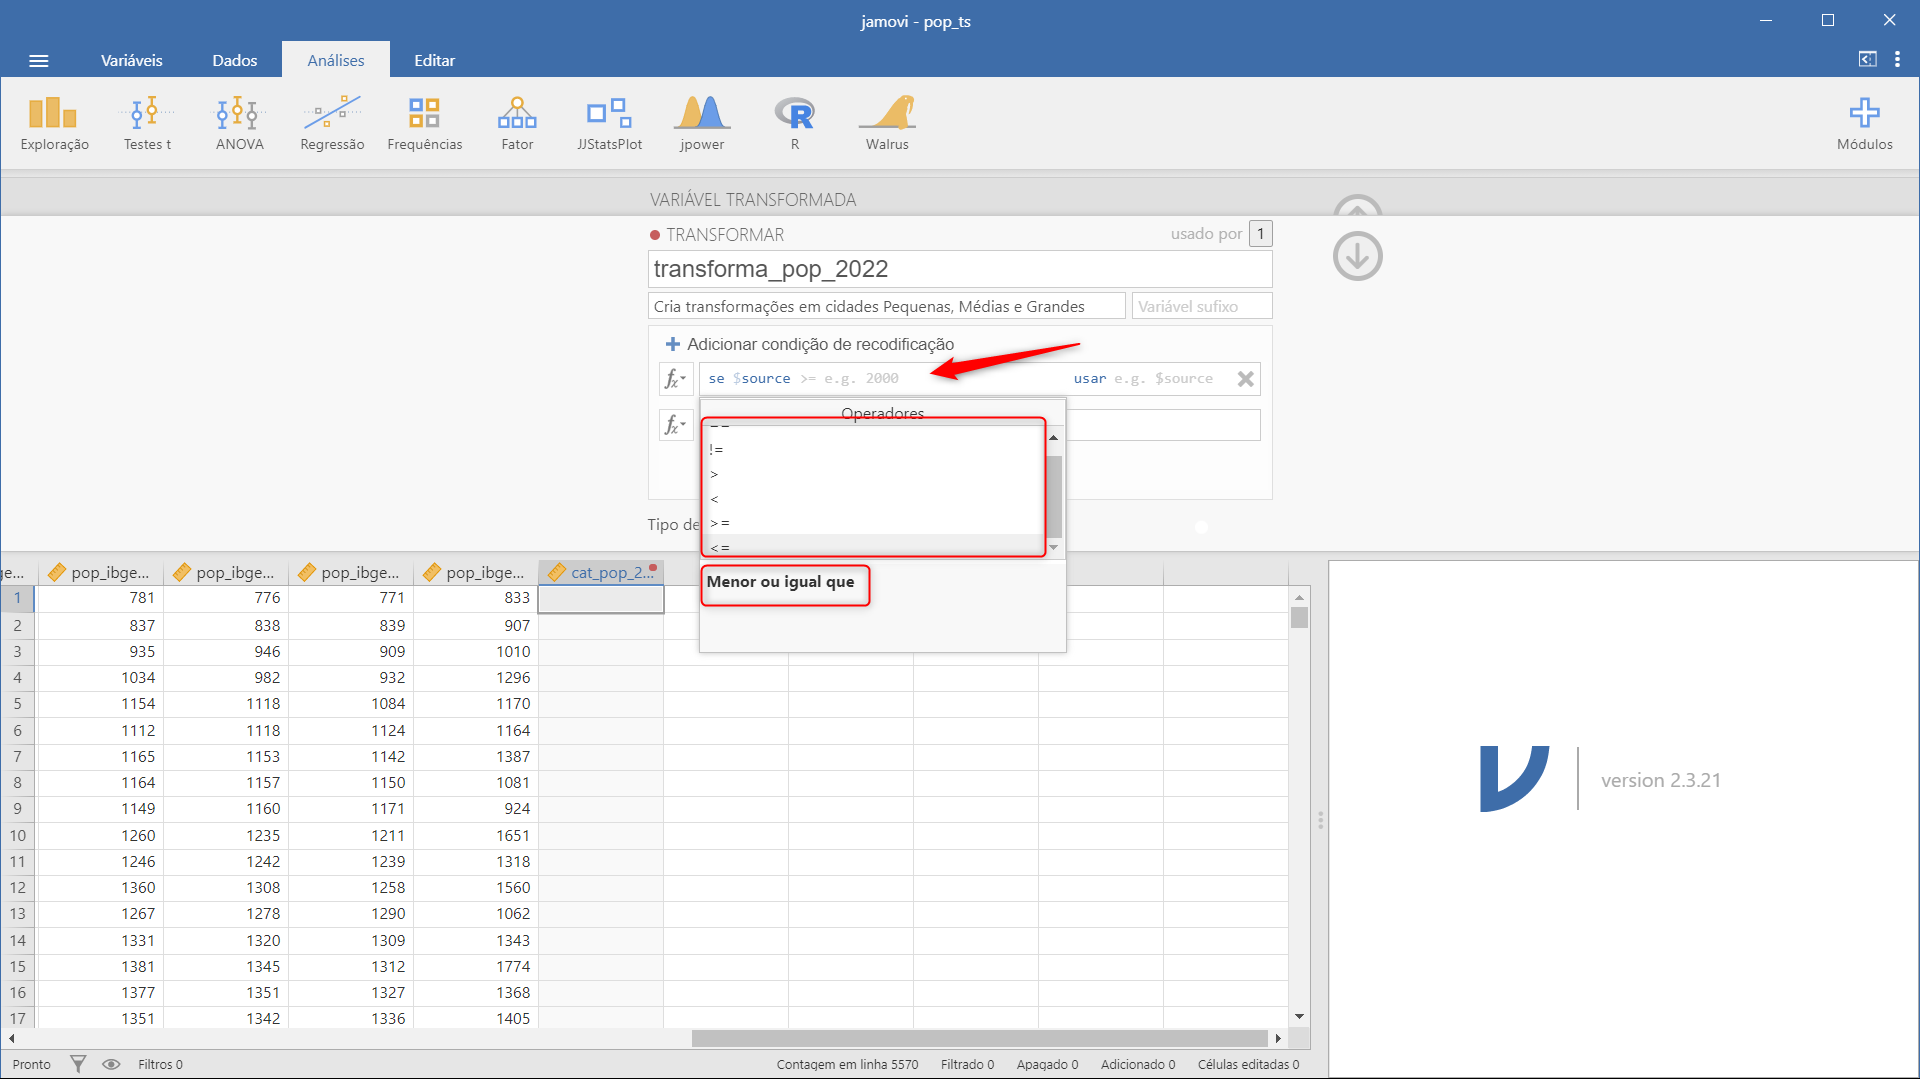
\includegraphics[width=\textwidth]{imagens/cap_2/criar_categoria_jamovi_5.png}
    \label{fig:criar_categoria_jamovi_5}
\end{figure}

Vamos entender a lógica que o Jamovi utiliza para criar categorias. O Jamovi avalia as condições em sequência, considerando a condição anterior. Por exemplo, ao definir a cidade pequena como sendo aquela com população menor ou igual a 20.000, basta escrever <= 20000. Ao prosseguir para a classificação das cidades médias, escrevemos <= 100000. O Jamovi, automaticamente, entende que esta condição deve ser contada a partir de 20.001 até 100.000, dado que a classificação anterior já contemplou as cidades com população menor ou igual a 20.000.

Na última condição, vamos utilizar o operador ELSE para definir as cidades grandes, pois agora só restam elas a serem classificadas. 

A Figura \ref{fig:criar_categoria_jamovi_6} mostra os 4 passos. Os três primeiros passos são as definições das condições de transformação e a quarta etapa é a verificação.

Um recurso interessante do Jamovi é que, enquanto você configura as transformações, o software automaticamente começa a criar as categorias para você, permitindo visualizar em tempo real se a recodificação está ocorrendo corretamente. 

\begin{figure}[H]
    \centering
    \caption{Criando as condições para Transformação de Variáveis}
    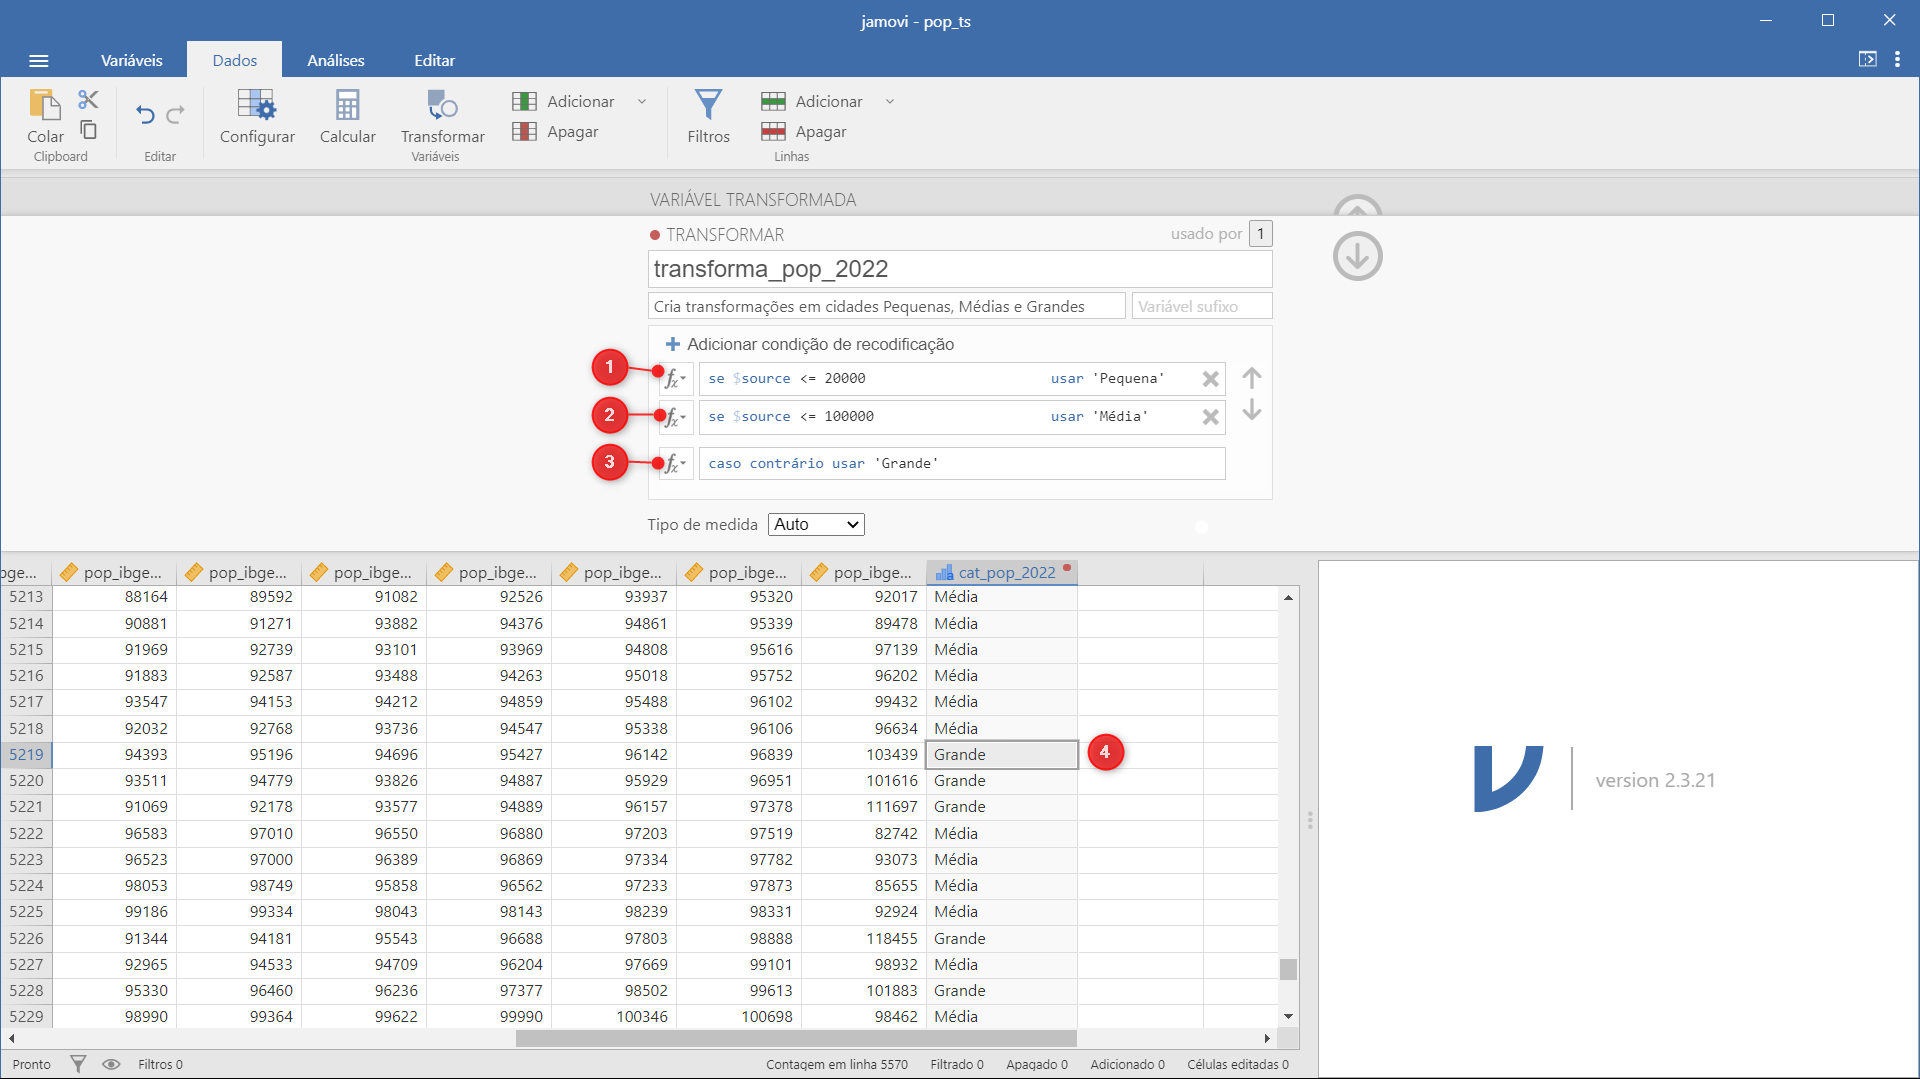
\includegraphics[width=\textwidth]{imagens/cap_2/criar_categoria_jamovi_6.png}
    \label{fig:criar_categoria_jamovi_6}
\end{figure}

Em nosso exemplo, nós escrevemos os nomes ``Pequena'', ``Média'' e ``Grande'' diretamente entre aspas, pois, relembrando, o Jamovi possui muitos componentes herdados da linguagem R. A linguagem R, assim como muitas outras linguagens de programação, usa aspas para designar textos. Portanto, sempre que quisermos definir uma categoria com um nome de texto, devemos colocar esse nome entre aspas.

Se você quiser criar categorias com códigos numéricos, as etapas são as mesmas, mas você deve utilizar números sem aspas. Por exemplo, poderíamos codificar ``Pequena'' como 1, ``Média'' como 2 e ``Grande'' como 3. Nesse caso, ao invés de escrever ``Pequena'', ``Média'' e ``Grande'' nas condições, escreveríamos os números correspondentes.

É importante lembrar que, ao usar códigos numéricos, será necessário criar uma legenda para lembrar o que cada número significa. Jamovi permite que você faça isso através de ``Níveis de Variáveis''.

Com a definição de todas as condições, a variável categórica está pronta para ser utilizada em suas análises. Como você pode ver, o processo de transformar uma variável contínua em uma variável categórica é bastante simples e intuitivo no Jamovi.

Para consolidar esse aprendizado, sugerimos que pratique o processo de criação de categorias com outros conjuntos de dados e exemplos. Lembre-se, a prática é uma parte importante do aprendizado. Quanto mais você praticar, mais natural o processo se tornará.

\section{Tratamento de Dados Faltantes}
Dados faltantes ou incompletos são uma realidade em análise de dados. Nesta seção, ensinaremos como identificar e tratar esses dados no Jamovi.

\section{Filtragem de Dados}
A filtragem é um passo crucial na preparação dos dados. Aqui, mostraremos como selecionar e filtrar subconjuntos de dados no Jamovi.

\section{Ordenação de Dados}
Nesta seção, abordaremos a ordenação de dados, uma operação importante para a visualização eficaz e análise de conjuntos de dados.

\section{Renomear e Reorganizar Variáveis}
Aqui, falaremos sobre como renomear e reorganizar variáveis no Jamovi. Esses são passos fundamentais na organização dos dados para análise.

\section{Dicas e Truques}
Esta seção apresentará dicas e truques úteis para melhorar a eficiência na manipulação de dados no Jamovi. Buscaremos compartilhar os melhores métodos e práticas recomendadas.

\section{Resumo do Capítulo}
Concluiremos o capítulo com um resumo, relembrando os principais tópicos abordados e reforçando os conceitos chave aprendidos sobre manipulação de dados no Jamovi.
